\documentclass[../competing_bandits_with_appendix.tex]{subfiles}
\begin{document}
\section{Competition and Better MAB Algorithms}\label{sec:competition}

% latex table generated in R 3.4.0 by xtable 1.8-2 package
% Thu Aug 16 13:13:01 2018
\begin{table*}[t]
\centering
\begin{tabular}{|c|c|c|c||c|c|c|}
  \hline
  & \multicolumn{3}{c||}{Heavy-Tail}
  & \multicolumn{3}{c|}{Needle-in-Haystack}\\
  \hline
  & $T_0$ = 20 & $T_0$ = 250 & $T_0$ = 500
  & $T_0$ = 20 & $T_0$ = 250 & $T_0$ = 500 \\
  \hline
\TS vs \DG
  & \makecell{\textbf{0.29} $\pm$0.03\\ \Eeog 55 (0)}
  & \makecell{\textbf{0.72} $\pm$0.02\\ \Eeog 570 (0)}
  & \makecell{\textbf{0.76} $\pm$0.02\\ \Eeog 620 (99)}
  %%
  & \makecell{\textbf{0.64} $\pm$0.03\\ \Eeog 200 (27)}
  & \makecell{\textbf{0.6} $\pm$0.03\\ \Eeog 370 (0)}
  & \makecell{\textbf{0.64} $\pm$0.03\\ \Eeog 580 (122)}
  \\
\hline
  $\TS$ vs $\DEG$
  & \makecell{\textbf{0.3} $\pm$0.03\\ \Eeog 37 (0)}
  & \makecell{\textbf{0.88} $\pm$0.01\\ \Eeog 480 (0)}
  & \makecell{\textbf{0.9} $\pm$0.01\\ \Eeog 570 (114)}
  %%
  & \makecell{\textbf{0.57} $\pm$0.03\\ \Eeog 150 (14)}
  & \makecell{\textbf{0.52} $\pm$0.03\\ \Eeog 460 (79)}
  & \makecell{\textbf{0.56} $\pm$0.02\\ \Eeog 740 (628)}
  \\
\hline
  $\DG$ vs $\DEG$
  & \makecell{\textbf{0.62} $\pm$0.03\\ \Eeog 410 (7)}
  & \makecell{\textbf{0.6} $\pm$0.02\\ \Eeog 790 (762)}
  & \makecell{\textbf{0.57} $\pm$0.03\\ \Eeog 730 (608)}
  %%
  & \makecell{\textbf{0.46} $\pm$0.03\\ \Eeog 340 (129)}
  & \makecell{\textbf{0.42} $\pm$0.02\\ \Eeog 650 (408)}
  & \makecell{\textbf{0.42} $\pm$0.02\\ \Eeog 690 (467)}
  \\
   \hline
\end{tabular}
\caption{{\bf Permanent duopoly}, for Heavy-Tail and Needle-in-Haystack instances. Each cell describes a game between two algorithms, call them Alg1 vs. Alg2, for a particular value of the warm start $T_0$. Line 1 in the cell is the market share of Alg 1: the average (in bold) and the 95\% confidence band.
%For example, the cell in the top left indicates that TS gets on average 64\% of the market when played against DG.
Line 2 specifies the ``effective end of game" (\Eeog): the average and the median (in brackets). The time horizon is $T=2000$.}
\label{sim_table}
\end{table*}

Our main experiments are with the duopoly game defined in Section~\ref{sec:model}. As the ``intensity of competition" varies from permanent monopoly to ``incumbent" to permanent duopoly to ``late entrant", we find a stylized inverted-U relationship as in Figure~\ref{fig:inverted-U}. More formally, we look for equilibria in the duopoly game, where each firm's choices are limited to \DG, \DEG and \TS. We do this for each ``intensity level" and each MAB instance, and look for findings that are consistent across MAB instances. For cleaner results, we break ties towards less advanced algorithms (as they tend to have lower adoption costs \cite{MWT-WhitePaper-2016,DS-arxiv}). Note that \DG is trivially the dominant strategy under permanent monopoly.

%(1) Permanent monopoly - indifferent between all algorithms but break indifference towards DG cause of deployment costs
%(2) Temporary monopoly - TS is the dominant strategy for the incumbent
%(3) Permanent duopoly -
%   (a) Under NIH, TS is dominant
%   (b) Under Heavy Tail, DG is weakly dominant
%   (c) Under Uniform, DG "beats" TS, but DEG "beats" TS by more than DG and DEG vs DG leads to ~50% market share (it's slightly in favor of DG but 50/50 is within the confidence band). If we break indifference towards DG cause of deployment costs, then we have that the unique PSNE is (DG, DG). If we don't add the indifference breaking, then we have four PSNE, (DG, DEG), (DEG, DG), (DG, DG), (DEG, DEG)


\subsubsection{Permanent duopoly.}
The basic scenario is when both firms are competing from round $1$. A crucial distinction is whether an MAB instance is exploration-disadvantaged:

\begin{finding}\label{find:duopoly}
\textit{Under permanent duopoly:
\begin{itemize}
\item[(a)] (\DG,\DG) is the unique pure-strategy Nash equilibrium for exploration-disadvantaged MAB instances with a sufficiently small ``warm start".
\item[(b)] This is not necessarily the case for MAB instances that are not exploration-disadvantaged. In particular, \TS is a weakly dominant strategy for Needle-in-Haystack.
\end{itemize}
}
\end{finding}


%\begin{finding}
%\textit{For sufficiently low warm start under the instances that are exploration-disadvantaged, the unique incentivized strategies in the competition game are:\footnote{The uniqueness comes from the fact that we break indifferences towards easier to deploy algorithms}
%\begin{center}
%\textbf{Permanent Monopoly} - $\DG$ \\
%\textbf{Temporary Monopoly} (incumbent)- $\TS$ \\
%\textbf{Permanent Duopoly} - $(\DG, \DG)$ \\
%\end{center}
%The conditions on $\TS$ being dominant under the temporary monopoly are that the incumbent is a temporary monopoly for sufficiently many periods.}
%\end{finding}

%\xhdr{Permanent Monopoly.} Since there is only a single firm in the
%market for the entire period, the firm can take the entire market
%regardless of what algorithm it deploys. \swedit{Since we assume that exploration algorithms ($\DEG$ and $\TS$) would incur deployment cost and firms break indifferences towards easier to deploy algorithms}, the firm would choose to deploy $\DG$.

We investigate the firms' market shares when they choose different algorithms (otherwise, by symmetry both firms get half of the agents). We report the market shares for Heavy-Tail and Needle-in-Haystack instances in Table \ref{sim_table}  (see the first line in each cell), for a range of values of the warm start $T_0$. Table~\ref{tab:duopoly_unif} reports similarly on the Uniform instance. We find that $\DG$ is a weakly dominant strategy for the Heavy-tail and Uniform instances, as long as $T_0$ is sufficiently small. However, \TS is a weakly dominant strategy for the Needle-in-Haystack instance. We find that for a sufficiently small $T_0$, \DG yields more than half the market against \TS,  but achieves similar market share vs. \DG and \DEG. By our tie-breaking rule, (\DG,\DG) is the only pure-strategy equilibrium.


\begin{table}[h]
\centering
\begin{tabular}{|c|c|c|c|}
 % \hline
 % & \multicolumn{3}{c|}{Uniform} \\
\hline
   & $T_0$ = 20 & $T_0$ = 250 & $T_0$ = 500 \\ \hline
\TS vs \DG
  & \makecell{\textbf{0.46} $\pm$0.03}
    & \makecell{\textbf{0.52} $\pm$0.02}
    & \makecell{\textbf{0.6} $\pm$0.02} \\ \hline
\TS vs \DEG
    & \makecell{\textbf{0.41} $\pm$0.03}
    & \makecell{\textbf{0.51} $\pm$0.02}
    & \makecell{\textbf{0.55} $\pm$0.02} \\ \hline
\DG vs \DEG
    & \makecell{\textbf{0.51} $\pm$0.03}
    & \makecell{\textbf{0.48} $\pm$0.02}
    & \makecell{\textbf{0.45} $\pm$0.02} \\\hline
\end{tabular}
\caption{{\bf Permanent duopoly}, for the Uniform MAB instance. Semantics are the same as in Table \ref{sim_table}.}
\label{tab:duopoly_unif}
\end{table}


\OMIT{This establishes our claim that $\DG$ is the incentivized algorithm.\footnote{We defer the table for uniform instances to the appendix. Summarizing the results, we see that, for low warm start, \DG yields more than half the market against \TS but is indifferent between \DG and \DEG. Since we break indifference towards easier to deploy algorithms, we also find that \DG is the incentivized algorithm in equilibrium}}

We attribute the prevalence of \DG on exploration-disadvantaged MAB instances to its prevalence on the initial ``exploration disadvantage period", as described in Section~\ref{sec:isolation}. Increasing the warm start length $T_0$ makes this period shorter: indeed, considering relative reputation trajectory in Figure~\ref{relative_rep_plots} (top), increasing $T_0$ effectively shifts the starting time point to the right. This is why it helps \DG if $T_0$ is small.


\OMIT{
The reason we see that $\DG$ is incentivized under the Heavy Tail and Uniform instances but that $\TS$ is weakly dominant under Needle In Haystack is precisely due to the fact that the purposeful exploration engaged by $\TS$ in the early rounds puts it in a disadvantage in the former case but not in the latter. Looking at the relative reputation plots in Figure \ref{relative_rep_plots}, we can interpret fixing a warm start $T_0$ as fixing the starting point on the relative reputation plots. The proportion of first rounds in the competition game that will go to a firm playing alg $A$ over a firm playing alg $B$ will correspond to the relative reputation proportion at time $T_0$. As a result, we see that for warm start $T_0 = 20$ on the exploration-disadvantaged instances, $\DG$ will win the first agent in a larger proportion of the simulations than $\TS$. However, on the Needle In Haystack instances, we see that $\TS$ wins a larger proportion of the first agents compared to $\DG$.
}

\subsubsection{Temporary Monopoly.}
We turn our attention to the temporary monopoly scenario. Recall that the incumbent firm enters the market and serves as a monopolist until the entrant firm enters at round $X$. We make $X$ large enough, but still much smaller than the time horizon $T$. We find that the incumbent is incentivized to choose \TS, in a strong sense:

\begin{finding}\label{find:temp-monopoly}
\textit{Under temporary monopoly, \TS is the dominant strategy for the incumbent. This holds across all MAB instances, if $X$ is large enough.
}
\end{finding}

The simulation results for the Heavy-Tail MAB instance are reported in Table~\ref{tab:ht-incum}, for a particular $X=200$. We see that \TS is a dominant strategy for the incumbent. Similar tables for the other MAB instances and other values of $X$ are reported in the supplement, with the same conclusion.

\begin{table}[H]
\centering
\begin{tabular}{|c|c|c|c|}
\hline
   & $\TS$  & $\DEG$  & $\DG$ \\ \hline
$\TS$
    & \makecell{\textbf{0.003}$\pm$0.003}
    & \makecell{\textbf{0.083}$\pm$0.02}
    & \makecell{\textbf{0.17}$\pm$0.02} \\\hline
$\DEG$
    & \makecell{\textbf{0.045}$\pm$0.01}
    & \makecell{\textbf{0.25}$\pm$0.02}
    & \makecell{\textbf{0.23}$\pm$0.02} \\\hline
$\DG$
    & \makecell{\textbf{0.12}$\pm$0.02}
    & \makecell{\textbf{0.36}$\pm$0.03}
    & \makecell{\textbf{0.3}$\pm$0.02} \\\hline
\end{tabular}
\caption{{\bf Temporary monopoly}, with $X=200$ (and $T_0=20$), for the Heavy-Tail MAB instance. Each cell describes the duopoly game between the entrant's algorithm (the row) and the incumbent's algorithm (the column). The cell specifies the entrant's market share (fraction of rounds in which it was chosen) for the rounds in which he was present. We give the average (in bold) and the 95\% confidence interval. NB: smaller average is better for the incumbent.}
\label{tab:ht-incum}
\end{table}
\OMIT{
\begin{table}[h]
\centering
\caption{Heavy Tail}
\begin{tabular}{|c|c|c|c|}
\hline
   & $\TS$  & $\DEG$  & $\DG$ \\ \hline
$\TS$
    & \makecell{\textbf{0.50, 0.50}}
    & \makecell{\textbf{0.3, 0.7}}
    & \makecell{\textbf{0.29, 0.71}} \\\hline
$\DEG$
    & \makecell{\textbf{0.7, 0.3}}
    & \makecell{\textbf{0.50, 0.50}}
    & \makecell{\textbf{0.38, 0.62}} \\\hline
$\DG$
    & \makecell{\textbf{0.71, 0.29}}
    & \makecell{\textbf{0.62, 0.38}}
    & \makecell{\textbf{0.50, 0.50}} \\\hline
\end{tabular}
\end{table}

\begin{table}[h]
\centering
\caption{Needle In Haystack}
\begin{tabular}{|c|c|c|c|}
\hline
   & $\TS$  & $\DEG$  & $\DG$ \\ \hline
$\TS$
    & \makecell{\textbf{0.50, 0.50}}
    & \makecell{\textbf{0.57, 0.43}}
    & \makecell{\textbf{0.64, 0.36}} \\\hline
$\DEG$
    & \makecell{\textbf{0.43, 0.57}}
    & \makecell{\textbf{0.50, 0.50}}
    & \makecell{\textbf{0.54, 0.46}} \\\hline
$\DG$
    & \makecell{\textbf{0.36, 0.64}}
    & \makecell{\textbf{0.43, 0.57}}
    & \makecell{\textbf{0.50, 0.50}} \\\hline
\end{tabular}
\end{table}
}


\DG is a weakly dominant strategy for the entrant, for Heavy-Tail instance in Table~\ref{tab:ht-incum} and the Uniform instance, but not for the Needle-in-Haystack instance. We attribute this finding to exploration-disadvantaged property of these two MAB instance, for the same reasons as discussed above.

\begin{finding}\label{find:temp-monopoly-entrant}
\textit{Under temporary monopoly, \DG is a weakly dominant strategy for the entrant for exploration-disadvantaged MAB instances.
}
\end{finding}

\subsubsection{Inverted-U relationship.}
We interpret our findings through the lens of the inverted-U relationship between the ``intensity of competition" and the ``quality of technology". The lowest level of competition is monopoly, when \DG wins out for the trivial reason of tie-breaking. The highest levels are permanent duopoly and ``late entrant". We see that \DG is incentivized for exploration-disadvantaged MAB instances. In fact, incentives for \DG get stronger when the model transitions from permanent duopoly to ``late entrant".%
\footnote{For the Heavy-Tail instance, \DG goes from a weakly dominant startegy to a strictly dominant one. For the Uniform instance, \DG goes from a Nash equilibrium strategy to a weakly dominant one.}
Finally, the middle level of competition, ``incumbent" in the temporary monopoly creates strong incentives for \TS. In stylized form, this relationship is captured in Figure~\ref{fig:inverted-U}.

% Transition Duopoly -> LateStart creates stronger incentives for DG.
% In Heavy Tail, DG is strictly dominant (before it was only weakly).
% In Uniform, DG is weakly dominant (before it was only PSNE).

Our intuition for why incumbency creates more incentives for exploration is as follows. During the temporary monopoly period, reputation costs of exploration vanish. Instead, the firm wants to improve its performance as much as possible by the time competition starts. Essentially, the firm only faces a classical explore-exploit tradeoff, and is incentivized to choose algorithms that are best at optimizing this tradeoff.

\subsubsection{Death spiral effect.}
Further, we investigate the ``death spiral" effect mentioned in the Introduction. Restated in terms of our model, the effect is that one firm attracts new customers at a lower rate than the other, and falls behind in terms of performance because the other firm has more customers to learn from, and this gets worse over time until (almost) all new customers go to the other firm. With this intuition in mind, we define  \textit{effective end of game} (\Eeog) for a particular \MRV and realization table, as the last round $t$ such that the agents at this and previous round choose different firms. Indeed, the game, effectively, ends after this round. We interpret low \Eeog as a strong evidence of the ``death spiral" effect. Focusing on the permanent duopoly scenario, we specify the \Eeog values in Table \ref{sim_table} (the second line of each cell). We find that the \Eeog values are indeed small:

\begin{finding}
\textit{
Under permanent duopoly, \Eeog values tend to be much smaller than the time horizon $T$.
}
\end{finding}

We also see that the \Eeog values tend to increase as the warm start $T_0$ increases. We conjecture this is because larger $T_0$ tends to be more beneficial for a better algorithm (as it tends to follow a better learning curve). Indeed, we know that the ``effective end of game" in this scenario typically occurs when a better algorithm loses, and helping it delays the loss.

\gaedit{
\subsubsection{Welfare}

\swedit{We also study the effects the competition has on the consumer
  welfare---the cumulative rewards received by the users over time.}
  
\begin{figure}
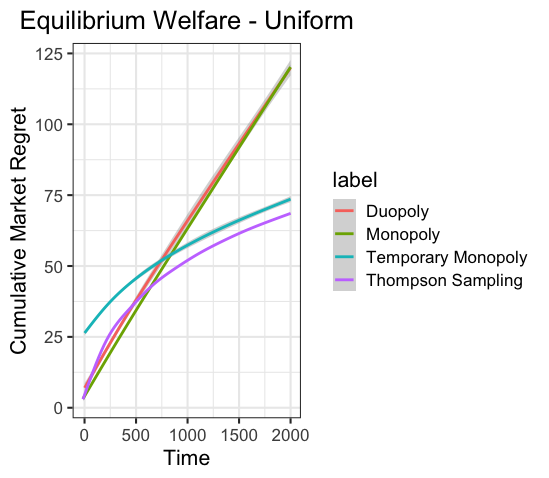
\includegraphics[scale=0.3]{figures/unif_eq_welfare}
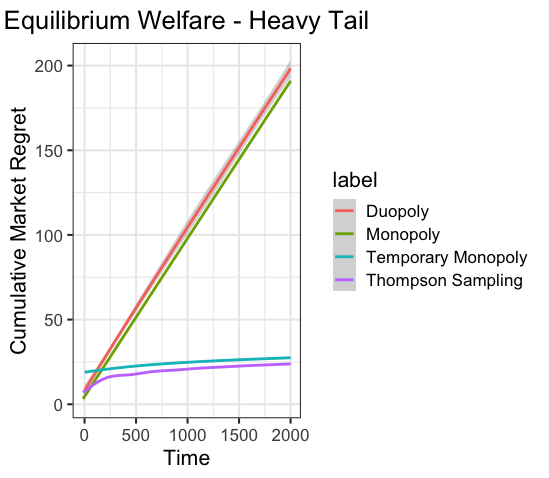
\includegraphics[scale=0.3]{figures/ht_eq_welfare}
\caption{Smoothed welfare plots resulting from equilibrium strategies in the different market structures. Note that welfare at $t = 0$ incorporates the regret incurred during the incumbent and warm start periods.}
\label{eq_regret}
\end{figure}

\begin{finding}
\textit{ \\ (a) Consumer welfare is highest under temporary monopoly. \\
(b) Increasing the number of firms in the market playing \DG weakly decreases consumer welfare.
}
\end{finding}

\swedit{For our purpose, it will be clearer to look at \emph{market
    regret}: the difference between the cumulative mean rewards
  achieved by taking the best action over all rounds and the
  cumulative mean rewards received by the agents. (Hence smaller
  regret means higher welfare.)}


Figure \ref{eq_regret} displays the \swedit{market regret (average
  over multiple runs)} under different levels of competitions,
assuming both firms playing their equilibrium strategies. Consumers are \textit{better off} in the temporary monopoly case than in
the duopoly case. However, this was expected from the fact that the incumbent is incentivized to play \TS. The welfare in the temporary monopoly case is close to the welfare to having a single firm playing
\TS.

\swedit{We also observe that monopoly and duopoly achieve similar
  welare, with monopoly being marginally better than duopoly. This is
  surprising since one might conjecture that the welfare should
  increase with the number of firms playing \DG since more $\DG$ runs
  should result in faster concentration on playing the better arms. In
  particular,, more firms playing \DG should result in faster
  discovery of a better arm, and the firm with such discovery would be
  able to attract more consumers and increase market welfare.}
\begin{figure}
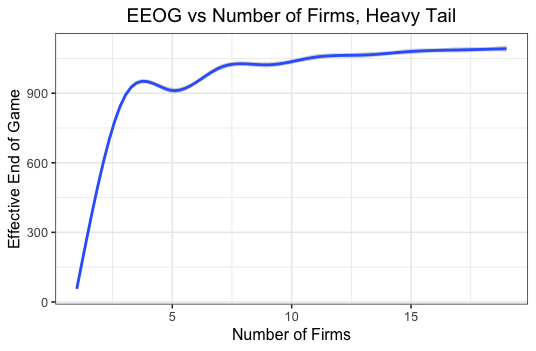
\includegraphics[scale=0.3]{figures/eeog_vs_num_ht}
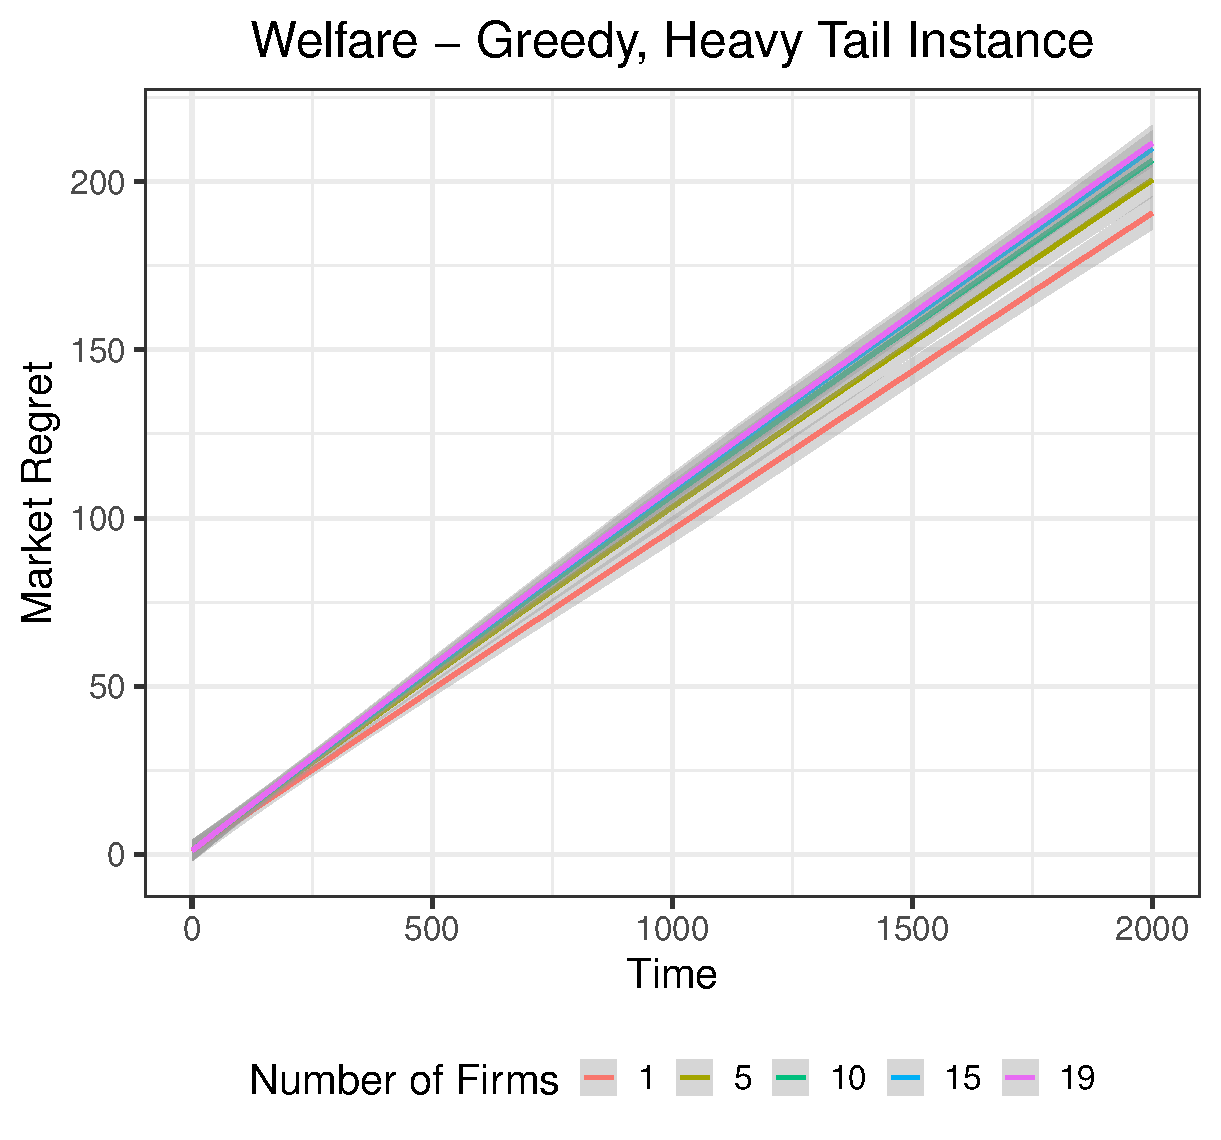
\includegraphics[scale=0.3]{figures/ht_many_firm_welfare}\\
\caption{Average welfare and EEOG as we increase the number of firms playing \DG}
\label{many_firm_welfare}
\end{figure}

\swedit{To study this phenomenon further, we go beyond the two-firm
  setting and simulate the game an increasing number of firms playing
  \DG.} Figure \ref{many_firm_welfare} reports the average welfare
across these simulations. Welfare not only does not get better,
\textit{but is weakly worse} as we increase the number of
firms. Correspondingly, we track the average \Eeog in each of the
simulations and notice that it is \textit{increasing} as the number of
firms increases. As we increase the number of firms, a single
individual firm gets fewer consumers for learning as consumers switch
between firms more often. Additionally, bad luck with rewards or arm
selection is punished even more harshly as we increase the number of
firms. This further strengthens the intuition from our previous
result, which is that learning may be hard under competition since
exploration and mistakes are punished harshly but are necessary for
learning.}


\end{document}
%%% Local Variables:
%%% mode: latex
%%% TeX-master: "../competing_bandits"
%%% End: 